% ============================================
% SEÇÃO 3.4: TRANSMISSÃO ATRAVÉS DE SISTEMAS LTI
% ============================================

\subsection{Sistemas Lineares Invariantes no Tempo}

\begin{frame}{O que é um Sistema LTI?}

Um \textbf{sistema} transforma um sinal de entrada $x(t)$ em um sinal de saída $y(t)$.

\begin{center}
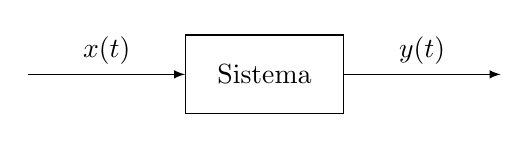
\begin{tikzpicture}[>=latex]
\node[draw, rectangle, minimum width=2cm, minimum height=1cm] (sys) at (0,0) {Sistema};
\draw[->] (-3,0) -- node[above] {$x(t)$} (sys.west);
\draw[->] (sys.east) -- node[above] {$y(t)$} (3,0);
\end{tikzpicture}
\end{center}

\vspace{0.3cm}

Um sistema é \textbf{Linear e Invariante no Tempo (LTI)} se possui duas propriedades:

\begin{enumerate}
\item \textbf{Linearidade:}
\[
x(t) = ax_1(t) + bx_2(t) \quad \Rightarrow \quad y(t) = ay_1(t) + by_2(t)
\]

\item \textbf{Invariância no tempo:}
\[
x(t - t_0) \quad \Rightarrow \quad y(t - t_0)
\]
\end{enumerate}

\textbf{Exemplos:} Filtros, amplificadores, canais de comunicação (sob condições ideais).

\end{frame}

% ============================================

\subsection{Resposta ao Impulso}

\begin{frame}{Resposta ao Impulso}

A \textbf{resposta ao impulso} $h(t)$ é a saída do sistema quando a entrada é $\delta(t)$:

\[
\delta(t) \quad \xrightarrow{\text{Sistema LTI}} \quad h(t)
\]

\textbf{Por que é importante?}

Qualquer sinal pode ser representado como soma de impulsos deslocados:
\[
x(t) = \int_{-\infty}^{\infty} x(\tau) \delta(t - \tau) d\tau
\]

Pela linearidade e invariância no tempo:
\[
y(t) = \int_{-\infty}^{\infty} x(\tau) h(t - \tau) d\tau = x(t) \conv h(t)
\]

\begin{block}{Relação Entrada-Saída no Tempo}
\[
\boxed{y(t) = x(t) \conv h(t)}
\]
\end{block}

\textbf{A resposta ao impulso caracteriza completamente um sistema LTI!}

\end{frame}

% ============================================

\subsection{Função de Transferência}

\begin{frame}{Função de Transferência (Resposta em Frequência)}

Aplicando a transformada de Fourier na relação $y(t) = x(t) \conv h(t)$:

\[
Y(\omega) = \FT{y(t)} = \FT{x(t) \conv h(t)}
\]

Pela propriedade de convolução:

\[
Y(\omega) = X(\omega) \cdot H(\omega)
\]

onde $H(\omega) = \FT{h(t)}$ é a \textbf{função de transferência} ou \textbf{resposta em frequência}.

\begin{block}{Relação Entrada-Saída na Frequência}
\[
\boxed{Y(\omega) = H(\omega) \cdot X(\omega)}
\]
\end{block}

\textbf{Vantagem:} Convolução no tempo $\rightarrow$ multiplicação na frequência!

A análise na frequência é muito mais simples.

\end{frame}

% ============================================

\begin{frame}{Interpretação da Função de Transferência}

\[
Y(\omega) = H(\omega) \cdot X(\omega)
\]

A função de transferência $H(\omega)$ é geralmente complexa:

\[
H(\omega) = |H(\omega)| e^{j\phi(\omega)}
\]

onde:
\begin{itemize}
\item $|H(\omega)|$: \textbf{ganho de magnitude} em cada frequência
\item $\phi(\omega) = \arg[H(\omega)]$: \textbf{mudança de fase} em cada frequência
\end{itemize}

\vspace{0.3cm}

\textbf{Efeito do sistema:}

\begin{itemize}
\item Cada componente de frequência de $X(\omega)$ é multiplicada por $|H(\omega)|$
\item A fase de cada componente é alterada por $\phi(\omega)$
\end{itemize}

\vspace{0.3cm}

\textbf{Aplicações:} Filtros selecionam/rejeitam certas frequências ajustando $|H(\omega)|$.

\end{frame}

% ============================================

\begin{frame}{Entrada Senoidal em Sistema LTI}

\textbf{Propriedade importante:} A resposta de um sistema LTI a uma entrada senoidal é também senoidal na mesma frequência.

Se $x(t) = A\cos(\omega_0 t + \theta)$, então:

\[
y(t) = A|H(\omega_0)| \cos(\omega_0 t + \theta + \phi(\omega_0))
\]

onde:
\begin{itemize}
\item Amplitude multiplicada por $|H(\omega_0)|$
\item Fase aumentada em $\phi(\omega_0)$
\item Frequência permanece $\omega_0$
\end{itemize}

\vspace{0.5cm}

\textbf{Demonstração:}

$x(t) = \Real\{Ae^{j(\omega_0 t + \theta)}\} = \Real\{Ae^{j\theta}e^{j\omega_0 t}\}$

Como $e^{j\omega_0 t} \xleftrightarrow{\ft} 2\pi\delta(\omega - \omega_0)$:

$y(t) = \Real\{Ae^{j\theta}H(\omega_0)e^{j\omega_0 t}\} = A|H(\omega_0)|\cos(\omega_0 t + \theta + \phi(\omega_0))$

\end{frame}

% ============================================

\subsection{Causalidade e Estabilidade}

\begin{frame}{Causalidade}

Um sistema é \textbf{causal} se a saída não depende de valores futuros da entrada:

\[
h(t) = 0 \quad \text{para} \quad t < 0
\]

\textbf{Significado físico:} Sistemas físicos reais são sempre causais (não podem "ver o futuro").

\vspace{0.3cm}

Para sistemas causais:
\[
y(t) = \int_{0}^{\infty} h(\tau) x(t - \tau) d\tau = \int_{-\infty}^{t} h(t - \tau) x(\tau) d\tau
\]

\vspace{0.3cm}

\textbf{Consequência na frequência:} A função de transferência $H(\omega)$ de um sistema causal satisfaz certas condições (critério de Paley-Wiener):

\[
\int_{-\infty}^{\infty} \frac{|\ln|H(\omega)||}{1 + \omega^2} d\omega < \infty
\]

Isso limita a rapidez com que $|H(\omega)|$ pode cair a zero.

\end{frame}

% ============================================

\begin{frame}{Estabilidade BIBO}

Um sistema é \textbf{BIBO estável} (Bounded Input, Bounded Output) se toda entrada limitada produz saída limitada.

\textbf{Critério de estabilidade:}

\[
\int_{-\infty}^{\infty} |h(t)| dt < \infty
\]

A resposta ao impulso deve ser absolutamente integrável.

\vspace{0.3cm}

\textbf{Na frequência:}

Para estabilidade BIBO, $H(\omega)$ deve existir e ser limitada:

\[
|H(\omega)| < \infty \quad \text{para todo} \quad \omega
\]

\vspace{0.3cm}

\textbf{Exemplos:}
\begin{itemize}
\item \textbf{Estável:} $h(t) = e^{-at}u(t)$ com $a > 0$
\item \textbf{Instável:} $h(t) = e^{at}u(t)$ com $a > 0$ (cresce exponencialmente)
\end{itemize}

\end{frame}

% ============================================

\subsection{Transmissão sem Distorção}

\begin{frame}{Condição para Transmissão sem Distorção}

\textbf{Objetivo:} Transmitir sinal sem alterar sua forma, apenas com ganho e atraso.

Desejamos:
\[
y(t) = K x(t - t_d)
\]

onde $K$ é um ganho constante e $t_d$ é um atraso fixo.

\vspace{0.3cm}

\textbf{Condição na frequência:}

Aplicando a transformada de Fourier:

\[
Y(\omega) = K X(\omega) e^{-j\omega t_d}
\]

Como $Y(\omega) = H(\omega)X(\omega)$:

\[
H(\omega)X(\omega) = K X(\omega) e^{-j\omega t_d}
\]

\end{frame}

% ============================================

\begin{frame}{Função de Transferência Ideal}

Para transmissão sem distorção:

\begin{block}{Condição de Transmissão sem Distorção}
\[
\boxed{H(\omega) = K e^{-j\omega t_d}}
\]
\end{block}

Isto significa:
\begin{itemize}
\item \textbf{Magnitude constante:} $|H(\omega)| = K$ para todas as frequências
\item \textbf{Fase linear:} $\phi(\omega) = -\omega t_d$ (proporcional a $\omega$)
\end{itemize}

\vspace{0.3cm}

\textbf{Interpretação física:}
\begin{itemize}
\item Todas as componentes de frequência têm mesmo ganho
\item Todas as componentes sofrem mesmo atraso $t_d$
\item A forma de onda é preservada
\end{itemize}

\vspace{0.3cm}

\textbf{Problema:} Sistemas reais não podem ter $|H(\omega)|$ constante para todo $\omega$ e serem causais simultaneamente!

\end{frame}

% ============================================

\subsection{Distorção em Sistemas}

\begin{frame}{Tipos de Distorção}

Quando $H(\omega) \neq K e^{-j\omega t_d}$, ocorre distorção:

\begin{enumerate}
\item \textbf{Distorção de Amplitude:}
   \begin{itemize}
   \item $|H(\omega)|$ não é constante
   \item Algumas frequências são amplificadas/atenuadas mais que outras
   \item Altera o formato do sinal
   \end{itemize}

\item \textbf{Distorção de Fase:}
   \begin{itemize}
   \item $\phi(\omega)$ não é linear com $\omega$
   \item Diferentes frequências sofrem atrasos diferentes
   \item Componentes chegam "fora de sincronia"
   \end{itemize}
\end{enumerate}

\vspace{0.3cm}

\textbf{Ambos os tipos degradam o sinal!}

Em sistemas práticos, busca-se minimizar distorção na banda de interesse.

\end{frame}

% ============================================

\begin{frame}{Atraso de Grupo}

O \textbf{atraso de grupo} quantifica o atraso de um "envelope" do sinal:

\[
\tau_g(\omega) = -\frac{d\phi(\omega)}{d\omega}
\]

\textbf{Interpretação:}
\begin{itemize}
\item Se $\phi(\omega) = -\omega t_d$ (linear), então $\tau_g = t_d$ (constante)
\item Se $\tau_g(\omega)$ varia, diferentes frequências têm atrasos diferentes
\item Causa distorção de fase
\end{itemize}

\vspace{0.3cm}

\textbf{Para transmissão sem distorção de fase:}

\[
\tau_g(\omega) = \text{constante}
\]

\vspace{0.3cm}

\textbf{Aplicação:} Importante em sinais modulados e pulsos digitais, onde o envelope carrega informação.

\end{frame}

% ============================================

\subsection{Largura de Banda}

\begin{frame}{Largura de Banda de Sistemas}

A \textbf{largura de banda} de um sistema mede a faixa de frequências que o sistema transmite eficientemente.

\textbf{Definições comuns:}

\begin{enumerate}
\item \textbf{Largura de banda de 3 dB:}
   \[
   |H(\omega)| \geq \frac{|H(\omega_{\max})|}{\sqrt{2}}
   \]
   Frequências onde o ganho cai no máximo 3 dB (metade da potência).

\item \textbf{Largura de banda de ruído:}
   \[
   B_n = \frac{1}{|H(\omega_{\max})|^2} \int_{-\infty}^{\infty} |H(\omega)|^2 d\omega
   \]

\item \textbf{Largura de banda absoluta:}
   
   Faixa onde $|H(\omega)| > 0$ (pode ser infinita).
\end{enumerate}

\textbf{Princípio:} Sistemas de banda limitada introduzem distorção em sinais de banda larga.

\end{frame}

% ============================================

\subsection{Exemplos de Sistemas LTI}

\begin{frame}{Exemplo 1: Filtro RC Passa-Baixas}

Circuito RC série com saída no capacitor:

\begin{center}
\begin{tikzpicture}[>=latex, american voltages]
% Entrada
\draw (0,0) -- (0,2);
\draw[<-] (0,2.2) -- (0,2.5) node[above] {$x(t)$};
% Resistor
\draw (0,2) -- (1,2);
\draw (1,1.5) rectangle (2,2.5) node[midway] {$R$};
\draw (2,2) -- (3,2);
% Capacitor
\draw (3,2) -- (3,1.5);
\draw (2.7,1.5) -- (3.3,1.5);
\draw (2.7,1) -- (3.3,1);
\draw (3,1) -- (3,0);
\node[right] at (3.3,1.25) {$C$};
% Terra
\draw (0,0) -- (3,0);
\draw (1.5,0) -- (1.5,-0.3) node[ground] {};
% Saída
\draw (3,1.25) -- (4,1.25);
\draw[->] (4,1.25) -- (4,1.75) node[above] {$y(t)$};
\end{tikzpicture}
\end{center}

\textbf{Equação diferencial:}
\[
RC\frac{dy(t)}{dt} + y(t) = x(t)
\]

\textbf{Transformada de Fourier:}
\[
RC \cdot j\omega Y(\omega) + Y(\omega) = X(\omega)
\]

\[
Y(\omega)[1 + j\omega RC] = X(\omega)
\]

\end{frame}

% ============================================

\begin{frame}{Exemplo 1: Função de Transferência do Filtro RC}

\[
H(\omega) = \frac{Y(\omega)}{X(\omega)} = \frac{1}{1 + j\omega RC}
\]

Definindo a \textbf{frequência de corte}: $\omega_c = 1/(RC)$

\[
H(\omega) = \frac{1}{1 + j\omega/\omega_c} = \frac{\omega_c}{\omega_c + j\omega}
\]

\textbf{Magnitude:}
\[
|H(\omega)| = \frac{1}{\sqrt{1 + (\omega/\omega_c)^2}}
\]

\textbf{Fase:}
\[
\phi(\omega) = -\arctan(\omega/\omega_c)
\]

\textbf{Características:}
\begin{itemize}
\item Em $\omega = 0$: $|H(0)| = 1$ (DC passa)
\item Em $\omega = \omega_c$: $|H(\omega_c)| = 1/\sqrt{2}$ (ponto de 3 dB)
\item Em $\omega \to \infty$: $|H(\omega)| \to 0$ (altas frequências atenuadas)
\end{itemize}

\end{frame}

% ============================================

\begin{frame}{Exemplo 1: Resposta em Frequência do Filtro RC}

\begin{center}
\includegraphics[width=\figFull, height=0.68\textheight, keepaspectratio]{figures/cap3/exponential_fourier}
\end{center}

\vspace{-0.3cm}
\begin{itemize}
\item A magnitude $|H(\omega)|$ é uma Lorentziana: máxima em DC, cai $-3\,\text{dB}$ em $\omega_c$
\item A fase $\phi(\omega) = -\arctan(\omega/\omega_c)$ é \textbf{não-linear} $\Rightarrow$ distorção de fase
\end{itemize}

\end{frame}

% ============================================

\begin{frame}{Exemplo 1: Resposta ao Impulso do Filtro RC}

A resposta ao impulso é a transformada inversa de $H(\omega)$:

\[
H(\omega) = \frac{\omega_c}{\omega_c + j\omega}
\]

Reconhecemos: $\frac{1}{a + j\omega} \xleftrightarrow{\ft} e^{-at}u(t)$

Portanto:

\[
h(t) = \omega_c e^{-\omega_c t} u(t) = \frac{1}{RC} e^{-t/(RC)} u(t)
\]

\textbf{Propriedades:}
\begin{itemize}
\item Causal: $h(t) = 0$ para $t < 0$
\item Estável: $\int_0^{\infty} h(t)dt = 1 < \infty$
\item Decai exponencialmente com constante de tempo $\tau = RC$
\end{itemize}

\textbf{Interpretação física:} O capacitor "suaviza" mudanças rápidas (altas frequências).

\end{frame}

% ============================================

\begin{frame}{Exemplo 2: Filtro Ideal Passa-Baixas}

Um filtro passa-baixas ideal tem função de transferência:

\[
H(\omega) = \begin{cases}
1 & |\omega| \leq \omega_c \\
0 & |\omega| > \omega_c
\end{cases} = \rect\left(\frac{\omega}{2\omega_c}\right)
\]

\textbf{Resposta ao impulso:}

Pela dualidade, sabemos que $\rect(t/\tau) \xleftrightarrow{\ft} \tau\sinc(\omega\tau/2\pi)$

Aplicando dualidade inversa:

\[
h(t) = \frac{\omega_c}{\pi} \sinc\left(\frac{\omega_c t}{\pi}\right) = \frac{\sin(\omega_c t)}{\pi t}
\]

\textbf{Problema:} $h(t) \neq 0$ para $t < 0$ $\rightarrow$ \textbf{não-causal}!

Filtro ideal passa-baixas é fisicamente irrealizável.

\end{frame}

% ============================================

\begin{frame}{Exemplo 2: Por que o Filtro Ideal é Irrealizável?}

\[
h(t) = \frac{\sin(\omega_c t)}{\pi t}
\]

\textbf{Problemas:}

\begin{enumerate}
\item \textbf{Não-causalidade:}
   \begin{itemize}
   \item $h(t) \neq 0$ para todo $t < 0$
   \item Sistema responde antes do impulso ser aplicado!
   \item Violação da causalidade física
   \end{itemize}

\item \textbf{Duração infinita:}
   \begin{itemize}
   \item $h(t)$ não decai a zero em tempo finito
   \item Oscila indefinidamente como $1/t$
   \item Impossível implementar exatamente
   \end{itemize}
\end{enumerate}

\vspace{0.3cm}

\textbf{Solução prática:} Usar filtros aproximados (Butterworth, Chebyshev) que são causais e aproximam o comportamento ideal.

\end{frame}

% ============================================

\begin{frame}{Resumo da Seção 3.4}

\textbf{Conceitos fundamentais de sistemas LTI:}

\begin{itemize}
\item \textbf{No tempo:} $y(t) = x(t) \conv h(t)$
\item \textbf{Na frequência:} $Y(\omega) = H(\omega) X(\omega)$
\item Análise na frequência simplifica cálculos!
\end{itemize}

\vspace{0.3cm}

\textbf{Propriedades importantes:}

\begin{itemize}
\item Causalidade: $h(t) = 0$ para $t < 0$
\item Estabilidade BIBO: $\int|h(t)|dt < \infty$
\item Transmissão sem distorção: $H(\omega) = Ke^{-j\omega t_d}$
\end{itemize}

\vspace{0.3cm}

\textbf{Tipos de distorção:}

\begin{itemize}
\item Amplitude: $|H(\omega)|$ não constante
\item Fase: $\phi(\omega)$ não linear
\end{itemize}

\textbf{Próximo:} Filtros ideais versus práticos.

\end{frame}
